\documentclass{cmc}
\usepackage{makecell}
\usepackage{enumitem}
\usepackage{amsmath}

% \usepackage{subfig}
\begin{document}

\pagestyle{fancy}
\lhead{\textit{\textbf{Computational Motor Control, Spring 2024} \\
    Final project, Project 2, GRADED}} \rhead{Student \\ Names}

\section*{Student names: \ldots (please update)}

\textit{
  In the second part of the CMC project you will implement a firing rate controller of the zebrafish and incorporate stretch feedback to study a biologically realistic spinal neural circuits. \textbf{Prerequisites}: please make sure that you followed the installation instructions of Project 1 and followed the description of the zebrafish model and simulation run/metrics.
}

\textit{
  \textbf{\corr{Deadline for Project 2: Friday 07/06/2024 23:59}}
}

\textbf{Instructions}

\begin{itemize}
  \item \textit{
    Update this file (or recreate a similar one, e.g.\ in
    Word) to prepare your answers to the questions. Feel free to add text,
    equations and figures as needed. Hand-written notes, e.g.\ for the development
    of equations, can also be included e.g.\ as pictures (from your cell phone or
    from a scanner). The code of project 1 should contain exercise 1a to 1c.
  }
  \item \textit{ Please submit both the source file.
    (*.doc/*.tex) and a pdf of your document, as well as all the used and updated
    python code can be submitted in a single zipped file called \newline
    \corr{final\_report\_name1\_name2\_name3.zip} where name\# are the team
    member's last names.  \corr{Please submit only one report per team!}
  }
\end{itemize}


\section*{1. The mechanical model}\label{sec:mechanical}
In this section we remind the features of the zebrafish model (see also the Project 1 assigment).

The mechanical zebrafish model consists of $n_{links}=16$ links connected by $n_{joints}=15$
rotational yaw torques using an Ekeberg spring-mass-damper muscle model.

For each joint $i=0,...,14$, the model receives in input the left ($M_{L_i}$) and right ($M_{R_i}$)
activations from the muscle cells, and the current joint angle ($\theta_i$) and speed ($\Dot{\theta_i}$)
to compute the resulting output torque ($\tau_i$) via:

\begin{eqnarray}
\label{eq:electro_mechanical}
	\tau_i = \alpha_i M_{diff_i} + \beta_i(\gamma_i +M_{sum_i} )\theta_i + \delta_i \Dot{\theta_i} \\
    M_{diff_i} = (M_{L_i} - M_{R_i}) \\
    M_{sum_i} = (M_{L_i} + M_{R_i})
\end{eqnarray}
Where $\alpha_i$ is the active gain, $\gamma_i$ is the passive stiffness, $\beta_i$ is the active stiffness, $\delta_i$ is the damping coefficient. The Ekeberg muscle model is a rotational spring-damper system with the addition of a variable stiffness term $\beta (M_L+M_R) \theta_i$. The active term of the model acts an external torque $\alpha(M_L-M_R)$. The Ekeberg model parameters have already been optimized (you do not need to change them).


\section*{2. Setting the zebrafish model for carangiform swimming}\label{sec:carangiform}
In the Project 1 you actuated all the 15 joints in open loop using a wave controller. By actuating all these joints in this fashion you mimicked an anguilliform swimmer (Fig \ref{fig:carangiform}a), in which the entire body is flexible through its length, and is actuated by a traveling wave from head to tail. However, this characteristics of slender fishes, like the lamprey, but not the zebrafish. The wave actuation in the zebrafish is concentrated on the tail segments, with the rostral segments that largely remain still the transverse plane (called carangiform swimmer, Fig \ref{fig:carangiform}b).

\begin{figure}[ht]
  \centering 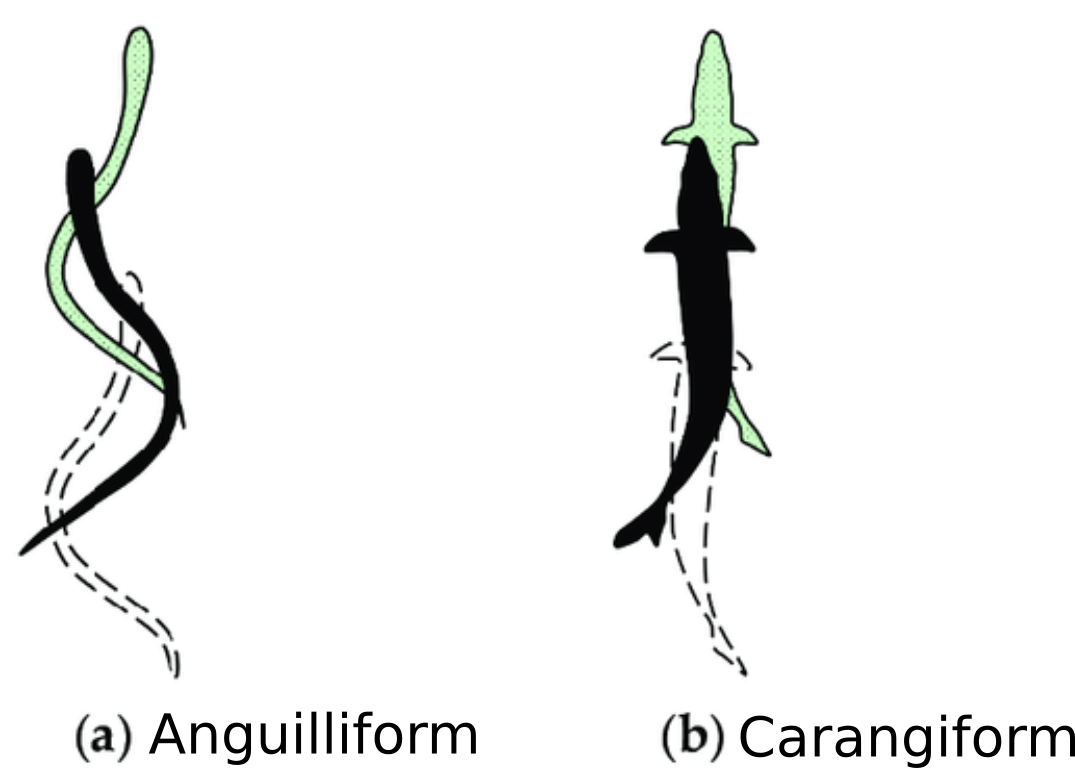
\includegraphics[width=0.5\textwidth]{figures/carangiform.png}
  \caption{\label{fig:carangiform} A snapshot of the body shape for an anguilliform (a) and carangiform (b) swimmer.}
\end{figure}

To model the carangiform swimming mode of the zebrafish in Project 2 you will only actuate joints $i=5,...,13$ by setting the remaining left and right muscle activations ($M_{L_i}$ and $M_{R_i}$, respectively) to zero (Fig \ref{fig:model_carangiform}).

\begin{figure}[ht]
  \centering 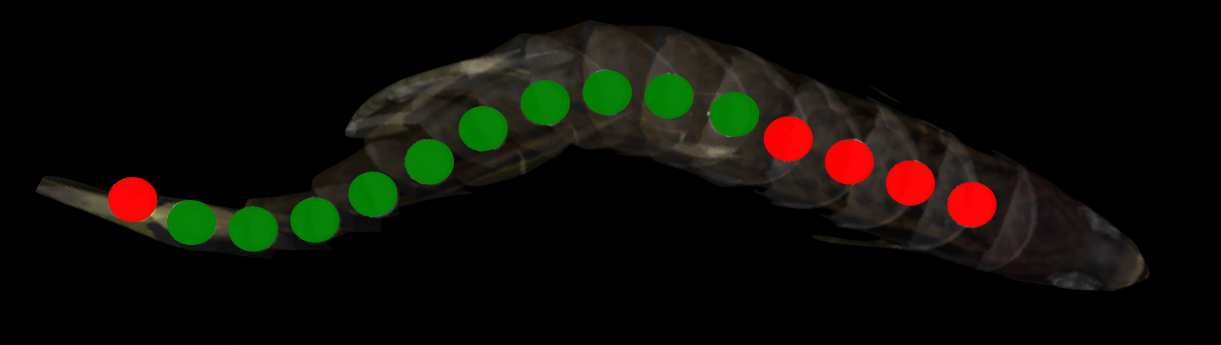
\includegraphics[width=0.5\textwidth]{figures/model_carangiform.png}
  \caption{\label{fig:model_carangiform} The joints in the zebrafish model that you should actively control in Project 2 (joints 5-13 green) and the ones that should be left passive (red, joints 0-4 and joint 14). }
\end{figure}


\section*{3. Overview of the firing rate neural network controller model}\label{sec:controller}

In this section we describe the equations of the neural network you will need to implement to control the zebrafish.

To model the spinal CPG controller, we consider two chains of $n_{cpg}=50$ populations of CPG neurons on each body side: one chain for the left side and one for the right side (blue circles in Fig \ref{fig:neural_diagram}), $n_{mc}=10$ populations of muscle cells on each side (MC, green circles in Fig \ref{fig:neural_diagram}, one for each of the 10 actuators), and $n_{ss}=50$ populations of stretch sensitive neurons on each side (SS, orange circles in Fig \ref{fig:neural_diagram}). Later we will introduce the connectivity scheme for these populations shown in Fig \ref{fig:neural_diagram}.

\begin{figure}[ht]
  \centering 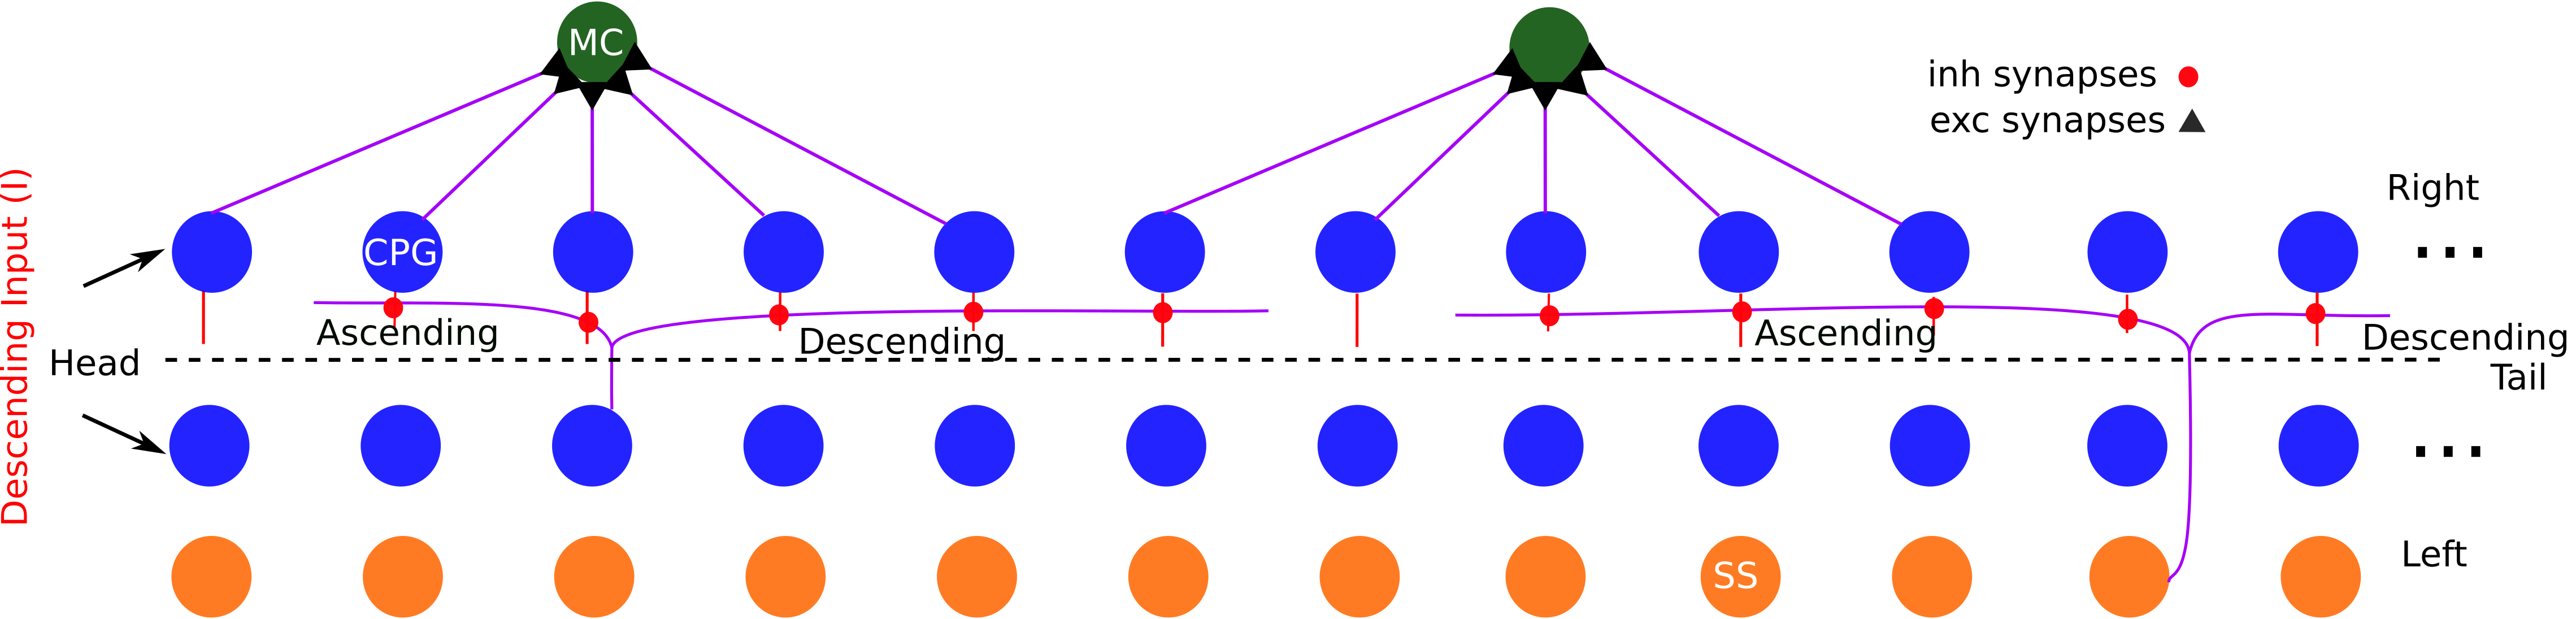
\includegraphics[width=1\textwidth]{figures/nn_diagram.png}
  \caption{\label{fig:neural_diagram} Neural controller diagram showing the sketch connectivity of the neural model. There are three neuron types: CPG neurons (CPG, in blue), muscle cells (MC, in green) and stretch sensory neurons (SS, in orange). Axons are shown in purple. Axons of SS and CPG neurons are commissural and have asceding and descending branches. CPG neurons are mainly descending (longer descending branch, i.e. more caudal connections), while SS neurons are ascending (longer ascending branch, i.e. more rostral connections). CPG neurons have axons that form excitatory synapses with muscle cells (five CPG neurons connect to 1 muscle cells). }
\end{figure}

\subsection*{The CPG population equations}

You will model each CPG unit using the firing rate equations with adaptation studied in Lab 4 (with no self-excitation). Let us index the units using the index $i=0,...,49$, then each left unit can be described by a pair of variables $(r_{L_i}, a_{L_i})$ ($(r_{R_i}, a_{R_i})$ for the right units), where $r_{L_i}$ represents the firing rate of the left CPG neuron $j$, and $a_{L_i}$ represents the firing rate adaptation (fatigue) of the left CPG neuron $j$.

\textit{Note: In lab 4 you used the same variables to define a two-unit circuit. Take inspiration from this lab to implement the controller in Project 2.
}

For simplicity, we assume that there is only one population of CPG neurons that is both inhibitory and excitatory (in reality, fishes have two or more separate classes of excitatory and inhibitory neurons. These receive input from other CPG populations on the chain, and from stretch sensory neurons.

We use the firing rate formalism to describe the activity of each CPG unit. Each CPG unit $i=0,...,49$ is described by the following pair of equations:

\begin{equation}
    \begin{array}{lcl}
	\tau \dot{r}_{L_i} = -r_{L_i} + F(I+I_{diff}-b a_{L_i} - g_{in} \sum_{j=0}^{49} w^{in}_{i,j} r_{R_i}  - g_{ss} \sum_{j=0}^{49} w^{ss}_{i,j} s_{R_i} \\
	\tau_a \dot{a}_{L_i} = -a_{L_i} + \rho r_{L_i} \\
	\tau \dot{r}_{R_i} = -r_{R_i} + F(I-I_{diff}-b a_{R_i} - g_{in} \sum_{j=0}^{49} w^{in}_{i,j} r_{L_i} \cdot \underline{r}_L - g_{ss} \sum_{j=0}^{49} w^{ss}_{i,j} s_{L_i} ) \\
	\tau_a \dot{a}_{R_i} = -a_{R_i} + \rho r_{R_i}.
    \end{array}
	\label{eq:neuron_equations}
\end{equation}

The biophysical meaning and default values of all parameters in Equation \ref{eq:neuron_equations} are given in Table \ref{table_par_CPG}. We assume that the system operates in the slow-fast regime, i.e. $\tau$ much smaller than $\tau_a$. This means that the neuron's spiking dynamics is faster than that of the firing adaptation, which is what is typically observed experimentally. The entries $w^{in}_{i,j}$ and $w^{ss}_{i,j}$ represent the connectivity matrices of CPG to CPG neurons and the one from stretch neurons to CPG neurons, respectively (defined in the next section).

The function $F=F(x)$ in Equation \ref{eq:neuron_equations} is called gain function, and it is the input-output non-linearity capturing the neural properties of the system. Here we will consider the following gain-function:
\begin{equation}
F=\sqrt{max(x,0)}.
\label{SReLu_eq}
\end{equation}


\begin{table}[h!]
\centering
\begin{tabular}{ l l l }
 Parameter & Meaning & Units \\
 $\tau=0.002$ & Neuron timescale & sec\\
 $\tau_a=0.3$ & Adaptation timescale & sec \\
 $b=10$ & Adaptation strength & - \\
 $g_{in}=2$ & CPG coupling strenth & -\\
 $g_{ss}=0$ & Stretch to CPG coupling strenth & -\\
 $I=10$ & Input current (i.e. from higher brain centers) & - \\
 $I_{diff}=0$ & Differential input (for turning) & - \\
 $\rho=0.5$ & Adaptation rate & -
\end{tabular}
\caption{Default values and biophysical meaning of the parameters of the firing rate CPG equations}
\label{table_par_CPG}
\end{table}


\subsection*{The muscle cell equations and conversion to muscle activations}

Each muscle cell and sensory neuron population activity is described by a single variable. For each $i=0,...,9$ the left (right) muscle cell $j$ is described by the variable $m_{L_i}$ ($m_{R_i}$). We model each muscle cell $i$ as a low-pass filter with activation and inactivation time scales $\tau^m_a=0.005 (sec)$ and $\tau^m_d=0.02 (sec)$ and strength $g_{mc}=0.3$, according to the following equations:

\begin{equation}
    \begin{array}{lcl}
	\dot{m}_{L_i} = g_{mc} \left[ \sum_{j=0}^{49} w^{mc}_{i,j} \cdot r_{L_j} \right] (1-m_{L_i}) / \tau^m_a - m_{L_i}/ \tau^m_d\\
	\dot{m}_{R_i} = g_{mc} \left[ \sum_{j=0}^{49} w^{mc}_{i,j} \cdot r_{R_j} \right] (1-m_{R_i}) / \tau^m_a - m_{R_i}/ \tau^m_d.
    \end{array}
	\label{eq:muscle_equations}
\end{equation}

In Equation \ref{eq:muscle_equations} the term $w^{ss}_{i,j}$ represents the connection weight from CPG neuron $j$ to muscle cell $i$ (described in the next section). The term $w^{mc}_{i,j}$  models the connectivity from CPGs to muscle cells (discussed in the next section). The term $(1-m_{L_i})$ in Equation \ref{eq:muscle_equations} guarantee that the muscle cell activities are bounded between 0 and 1.

The 20 muscle cells' activities described by Equation \ref{eq:muscle_equations} (10 activities per side) are then converted to the 10 active muscle activations in the Ekeberg equations \ref{eq:electro_mechanical} as a weight multiplication by a constant parameter $w_{act}=0.3$. For $j=0,...,9$ we therfore have:
\begin{equation}
    \begin{array}{lcl}
	M_{L_{j+4}} = w_{act} m_{L_i}\\
	M_{R_{j+4}} = w_{act} m_{R_i}
    \end{array}
	\label{eq:mc_activation_conversion}
\end{equation}
The remaining muscle activations are passive and you should set them to zero, i.e. $M_{L_{j}}=M_{R_{j}}=0$ for $j=0,1,2,3$ (the first 4 rostral joints) and $j=14$ (the tail joint).


\subsection*{The stretch sensory population equations}
In the second part of Project 2 you will study the effect of adding a stretch feedback loop in the firing rate controller. We already menioned that we consider 50 neurons that can sense stretch feedback angle positions. However, there are only 10 joints actively bending joints. Therefore, we will use interpolation at each time step iteration to interpolate the angle positions at 50 joint locations.

We assume that all sensors are uniformly distributed longitudinally along the positions of the first and last active joint (the vector of positions of the 50 joint sensors are already provided in \corr{firing\_-rate\_controller.py::FiringRateController.poses\_ext}). At each time step, you will need to compute the joint position $\theta_i$ at position $i$ by calling the interpolated positions of the 10 joint positions (accessed by the array pos in \corr{firing\_rate\_controller.py::-FiringRateController.ode\_rhs}) (you can use the CubicSpline function in the scipy library). The interpolation function at integration step $n$ as $INTERP_n$ for $i=0,...,49$ gives then the value of $\theta_i$ as:
$$ \theta_i = INTERP_n(poses_{ext_i}) $$

For each $i=0,...,49$ the left (right) stretch sensory neuron population $j$ is described by the variable $s_{L_i}$ ($s_{R_i}$). We model stretch sensory population $i$ as low-pass fiters for the interpolated stretch joint angle, similar to the muscle cell equations (but with a single timescale $\tau_{ss}=0.005$). Each sensory population variable evolves accoriding to:
\begin{equation}
    \begin{array}{lcl}
	\tau_{ss} \dot{s}_{L_i} = F(\theta_i) (1-s_{L_i}) - s_{L_i}\\
	\tau_{ss} \dot{s}_{R_i} = F(-\theta_i) (1-s_{R_i}) - s_{R_i}.
    \end{array}
	\label{eq:sensors_equations}
\end{equation}

\section*{4. Connectivity matrices}
Let us now define the connectivity matrices $W_{in}=(w^{in}_{i,j})$ (CPG to CPG connections), $W_{ss}=(w^{ss}_{i,j})$ (stretch to CPG connections) and $W_{cm}=(w^{ss}_{i,j})$ (CPG to MC connections) in Equations \ref{eq:neuron_equations}-\ref{eq:sensors_equations}. These represent the synaptic interactions of the units schematically represented in Fig \ref{fig:neural_diagram}. Descending and ascending axonal branches from the soma of pre-synaptic neurons project to the post-synaptic partners. The CPG neurons (or stretch neurons) form $n_{desc}$ connections to the closest caudal CPG cells and $n_{asc}$ connections to the closest rostral cells. The general connectivity matrix scheme for matrices $W_{in}$ and $W_{ss}$ is the following:
\begin{equation}
    w_{i,j} = \begin{cases}
      1/(j-i+1), \quad if \quad i \leq j \quad and \quad j-i \leq n_{desc}\\
      1/(i-j+1), \quad if \quad i>j \quad and \quad i-j \leq n_{asc}\\
      0, \quad otherwise
    \end{cases}
\end{equation}
For $i,j=0,...,49$. In this equation parameters $n_{desc}$ and $n_{asc}$ are different for $W_{in}$ and $W_{sc}$, taking inspiration from experiments on the real animal, where CPG connections were found to be primarily descending, while sensory to CPG connections primarily ascending \cite{picton_developmental_2022, picton_spinal_2021}. Therefore, for $W_{in}$ we choose primary we fix $n_{desc}=2$ and $n_{asc}=1$, while for $W_{sc}$ we fix $n_{desc}=0$ and $n_{asc}=10$.

The connectivity from CPGs to MCs is as shown in Figure \ref{fig:neural_diagram}. Each MC receives input from $n_{mc}=n_{cpg}/n_{muscle}=5$ CPG neurons. For each $j=0,...,49$ (pre-synaptic CPG cell), $i=0,...,9$ (post-synaptic MC cell) the connection weight is given by:
\begin{equation}
    w^{mc}_{i,j} = \begin{cases}
      1 \quad if \quad n_{mc} i \leq j \leq n_{mc} (i+1)-1\\
      0, \quad otherwise
    \end{cases}
\end{equation}

\subsection*{Vectorized computations}
To simulate the controller it is crucial that the operations you will implement to solver the system are properly vectorized using NumPy. Here are some tips to guide your implementation.

\textit{Notation:
Below we will make use of vectors in underscore $\underline{x}=(x_0,...,x_{n-1})$ notation, of the connectivity (weighted) matrix $W=(w_{i,j})_{0\leq i \leq m-1, \; \leq j \leq n-1}$, where $w_{i,j}$ represents the connection from unit $j$ to unit $i$, and of the matrix by vector multiplication operation
$$ \underline{y} = W \cdot \underline{x} $$
defined by:
$$ y_i = \sum_{j=0}^{n-1} W_{i,j} \cdot x_j $$
}

Let us use this notation to define the vectors of left (right) neuron activities as $\underline{r}_L=(r_{L_0},...,r_{L_{49}})$ ($\underline{r}_R=(r_{R_0},...,r_{R_{49}})$), the vector of left (right) muscle cell activities $\underline{m}_L=(m_{L_0},...,m_{L_9})$ ($\underline{m}_R=(m_{R_0},...,r_{R_9})$) and the vector of left (right) neuron activities as $\underline{s}_L=(s_{L_0},...,s_{L_{49}})$ ($\underline{s}_R=(s_{R_0},...,s_{R_{49}})$). Let us also define the vector of interpolated joint angles positions
$$\underline{\theta} = (INTERP_n(poses_{ext_0},...,INTERP_n(poses_{ext_{49}}))$$

Using this notation we can rewrite the entire closed loop system of equations \ref{eq:neuron_equations}-\ref{eq:sensors_equations} in the following vectorial form:

\begin{equation}
    \begin{array}{lcl}
	\tau \dot{\underline{r}}_{L} = -\underline{r}_L + F(I-b \underline{a}_L - g_{in} W_{in} \cdot \underline{r}_R - g_{ss} W_{ss} \cdot \underline{s}_R )\\
	\tau_a \dot{\underline{a}}_L = -\underline{a}_L + \rho \underline{r}_L \\
	\tau \dot{\underline{r}}_{R} = -\underline{r}_R + F(I-b \underline{a}_R - g_{in} W_{in} \cdot \underline{r}_L - g_{ss} W_{ss} \cdot \underline{s}_L )\\
	\tau_a \dot{\underline{a}}_R = -\underline{a}_R + \rho \underline{r}_R \\
	\dot{\underline{m}}_L = g_{mc} W_{mc} \cdot \underline{r}_L (1-\underline{m}_L) / \tau^m_a - \underline{m}_L/ \tau^m_d\\
	\dot{\underline{m}}_R = g_{mc} W_{mc} \cdot \underline{r}_R (1-\underline{m}_R) / \tau^m_a - \underline{m}_R/ \tau^m_d. \\
	\tau_{ss} \dot{\underline{s}}_L = F(\theta_i) (1-\underline{s}_L) - \underline{s}_L\\
	\tau_{ss} \dot{\underline{s}}_R = F(-\theta_i) (1-\underline{s}_R) - \underline{s}_R\\
    \end{array}
	\label{eq:equations_vectorial}
\end{equation}

You will need to implement this system in the function \corr{firing\_rate\_controller.py::ode\_rhs}. To properly vectorize these computations you will need to create index vectors for the different variables in the system (take inspiration from Lab 4).

For the initial conditions, for all variables are already set random initial conditions for you.

% \newpage

\subsection*{Code organization}\label{subsec:code}

In this exercise you will modify the files \fileref{exercise\_\#.py}, \fileref{firing\_rate\_controller.py}, \fileref{simulati\-on\_parameters.py} (optional) and \fileref{plot\_results.py} (optional). We provide below
a brief description of these and the other files, for completeness.

\begin{itemize}
\item \corr{\textbf{example\_single.py}} --- Run single simulation example (fixed parameters)
\item \corr{\textbf{example\_multiple.py}} --- Run multiple parallel simulations with different parameters
\item \corr{\textbf{exercise\_\#.py}} --- Files for the exercises 3-10
\item \corr{\textbf{firing\_rate\_controller.py}} --- Contains the equations for the firing rate neural controller. You have to implement here the differential equations.
\item \corr{\textbf{simulation\_parameters.py}} --- This file contains the
  SimulationParameters class and is provided for convenience to send parameters
  to the setup of the controller. Please carefully read the parameter list
  and their documentation in this code. We provided the names and default values of
  all the controller parameters (for simplicity). Use these parameters or create
  new ones to write the equations.
\item \corr{\textbf{metrics.py}} --- This file contains the implementation
  for all the controller/mechanical metrics (see below). Modified from Project 1.
\end{itemize}

The other files are the same as reported in the Assigment of Project 1.

\subsection*{Running the simulations}\label{subsec:simulating}
Follow the same instructions as in the previous Assignment (Project 1 Assignment). Use the test files \textbf{example\_single.py} and \textbf{example\_multiple.py} for running single and multiple simulations, respectively, similar to Project 1.


\subsection*{Additional tools: metrics and plotting}\label{subsec:plotting}
Feel free to use all the plotting tools and metrics explained in the Assigment of Project 1. In addition, we provided a new metric to compute the turning curvature of the fish (useful for Exercise 5):  \newline
\textbf{Curvature metric}. Stored in metrics["curvature"] (values $\in \mathbb{R}$). First we compute this metric by calculating the average frequency $f$ of the muscle difference signals $M_{diff_i}$ using the threshold crossing detection method. If $f>0$ (otherwise, the curvature is zero) it samples the center of mass trajectory in the x-y plane $(x(t),y(t))$ across subsequent cycles and computes inverse of the radius of curvature from this trajectory according to the following formula:

\begin{equation}
 \label{eq:curvature}
 \frac{x'' \cdot y' - x' \cdot y''}{(x'^2 + y'^2)^{3/2}}
\end{equation}
Where $'=d/dt$ and $''=d^2/dt^2$.

% \newpage


\subsection*{Final notes}
\begin{itemize}
\item Use the exercise files \fileref{exercise\_X.py}, with X the exercise number to answer the question X, for example, \fileref{exercise\_3.py} to answer question 3. \fileref{exercise\_X.py} should be used as a script to run the simulations and (optionally) plot the results.
\item Check the notes on the code. Many explanations are given therein.
\item Be concise and precise in the answers in the answers of the exercises.
\item You can append videos to explain your reasoning.
\end{itemize}



%%%%%%%%%%%%%%%%%%%%%%%%%%%%%%%%%%%%%%%%%%%%%%%%%%%%%%%%%%%%%%%%%%%%%%%%%%%%%%%%%%%%%%%%%%%%%%%%%%%
\newpage
\section*{5. Questions}
At this point you can now start to work on implementing your exercises 3-9 below (use \textbf{exercise3.py}-\textbf{exercise9.py} to solve the exercises).

\textit{Note: for the exercises 4 and 5 below you do not need to simulate the mechanical model, you can simply run the \fileref{run\_open\_loop.py} file that is already called in \fileref{exercise3.py} and \fileref{exercise4.py}. }

\subsection*{3. Implement the equations for the firing rate controller}\label{sec:ex3}
Implement the open loop firing rate controller in \ref{eq:equations_vectorial} without the feedback terms (omit the terms $g_{ss} W_{ss} \cdot \underline{s}_R$ and the sensory feedback neuron equations for $\dot{\underline{s}}_L$ and $\dot{\underline{s}}_R$). Run the network for fixed default parameters and plot the CPG and MC activities. Demonstrate that the network with default parameters supports an oscillatory traveling wave of activity propagating from the head to the tail and use the metrics to quantify frequency, amplitude, wavefrequency, ptcc.





%% -----------------------------SOLUTION ------------------------------


\subsection*{4. Explore the dependency on the descending input drive $I$}\label{sec:ex4}
The descending input parameter $I$ represents the excitation to the CPG network from higher brain centers. Vary $I \in \left[0,30 \right]$ in the system and test the ranges of descending inputs that support of oscillations (you can use the ptcc metric to measure the stability of the oscillations). How does the frequency and wavefrequency change within the range of $I$ that support the oscillations?




%% -----------------------------SOLUTION -----------------------------



\subsection*{5. Test the firing rate controller swimming behavior and turning}\label{sec:ex5}
In exercises 3 and 4 you have simulated the firing rate controller, but not the neuromechanical zebrafish model. Run an individual simulations with default parameters, visualize the swimming behavior and test its performance. Next, test the ability of the turning by applying a differential drive $I_{diff} \in \left[ 0,4 \right]$ (run a parameter sweep in this interval). To measure the turning performance, you can use the curvature and lateral speed metrics. Check that the turning radius match the curvature expected from the trajectory (i.e. plot the center of mass trajectory and the compute the radius=1/curvature). Plot a swimming trajectory and neuron activities for fixed $I_{diff}=0$ and $I_{diff}>0$. How does the activities of left and right CPGs and MCs change for the case $I_{diff}>0$?


%% -----------------------------SOLUTION ------------------------------



\subsection*{6. Implement the feedback equations and test different feedback weights}\label{sec:ex6}
Implement now the feedback equations and add stretch feedback to the CPG oscillators ($g_{ss} > 0$), i.e. implement the full network \ref{eq:equations_vectorial} and test the role of the stretch feedback to the controller for fixed parameters. Plot the activities of CPG neurons, muscle cells and sensory neurons and that of the joint angle positions. Now vary $g_{ss} \in \left[0,15 \right]$, how does the frequency, wavefrequency and forward speed change? Is feedback beneficial for a good swimming performance? Under which conditions?


%% -----------------------------SOLUTION ------------------------------


\subsection*{7. Explore the dependency on the descending input $I$ and feedback weight $g_{ss}$}\label{sec:ex7}
Repeat the analysis of question 5 for different values of $g_{ss} \in \left[0,15 \right]$. How does the frequency and wavefrequency change with the added feedback? Does the ranges of inputs $I$ leading to stable oscillation change? What about the performance (i.e. forward speed) for these ranges of $I$, does it change?


%% -----------------------------SOLUTION ------------------------------



\subsection*{8. Explore the effect of noise with/o feedback}\label{sec:ex8}
Let us now consider the effect of noise in the system and test the robustness of the network to noise. You will add noise to the activity variables of the CPG neurons in equation \ref{eq:equations_vectorial}. We consider two vector of Ornstein-Uhlenbeck processes $\underline{x}_t = (x_{t_0},...,x_{t_{49}})$ (for the left neurons) and $\underline{y}_t = (y_{t_0},...,y_{t_{49}})$ (for the right neurons):
\begin{equation}
    \begin{array}{lcl}
	d\underline{x}_t = - \theta \underline{x}_t \cdot dt + \sigma dW_t\\
	d\underline{y}_t = - \theta \underline{y}_t \cdot dt + \sigma dW_t\\
    \end{array}
	\label{eq:ou_process}
\end{equation}

Where $\theta>0$ and $\sigma>0$ are parameters, and $W_t$ is a Weiner process. Here, we choose $\theta=0.1$. The CPG activity equations in \ref{eq:equations_vectorial} will now be modified by adding the noise terms according to:

Implement in \corr{firing\_rate\_controller.py::-get\_ou\_noise\_process\_dw} an Euler-Maruyama scheme for solving numerically the Ornstein-Uhlenbeck process.

Internally (you do not need to implement this!), the solution of the Euler-Maruyama scheme will be added to the original system's variables to solve the CPG activities with added noise:
\begin{equation}
    \begin{array}{lcl}
	\tau \dot{\underline{r}}_{L} = -\underline{r}_L + F(I-b \underline{a}_L - g_{in} W_{in} \cdot \underline{r}_R - g_{ss} W_{ss} \cdot \underline{s}_R ) + \underline{x}_t\\
	\tau \dot{\underline{r}}_{R} = -\underline{r}_R + F(I-b \underline{a}_R - g_{in} W_{in} \cdot \underline{r}_L - g_{ss} W_{ss} \cdot \underline{s}_L ) + \underline{y}_t
    \end{array}
	\label{eq:noise_added_vectorial}
\end{equation}

Now that you have added the noise process in the system, run a two parameter search, varying $\sigma \in \left[0, 30\right]$ and $w_{stretch} \in \left[0, 10\right]$. Is the feedback helpful to stabilizing the oscillations and performance under noise (use the speed PCA metric to evaluate the performance, as it is less sensitive to the noise)?

\textit{Note: when adding noise in the system, you should not consider the frequency and wavefrequency metrics, as they could be corrupted by the noise.}

%% -----------------------------SOLUTION ------------------------------



\subsection*{9. Open question}\label{sec:ex9}
Open questions. These questions are meant to assess your understanding of the topics addressed during the project. You should reply in a concise, scientific way by explaining your reasoning and listing the reference literature to support your idea.

\begin{enumerate}
\item During the project, you tested the effect of proprioceptive sensory feedback with varying levels of noise. How would you design a biological experiment to validate in-vivo the simulation results?
\item What other aspects of zebrafish locomotion could be affected by the presence (or absence) of proprioceptive sensory feedback? How would you test those hypotheses in simulation and biological experiments?
\item What other types of sensory feedback could play a role during zebrafish locomotion? How would you disambiguate the relative contribution of the different sensory feedback modalities? How can simulation help in addressing this problem?
\end{enumerate}



%% -----------------------------SOLUTION ------------------------------


\bibliographystyle{ieeetr}
\bibliography{cmc_2024}
\label{sec:references}





% \newpage

% \section*{APPENDIX}
% \label{sec:appendix}

\end{document}

%%% Local Variables:
%%% mode: latex
%%% TeX-master: t
%%% End: